\chapter{Conceptual Design}
Ein erstes Design für die Benutzeroberfläche wurde mit dem Mock-Up Tool \textit{Balsamiq} entwickelt. Hierbei ging es primär darum Unstimmigkeiten und grobe Fehleinschätzungen auszumerzen, um anschließend einen funktionalen Prototypen entwickeln zu können. Mehr oder weniger parallel wurden auch schon Mock-Ups mit Hilfe von HTML erzeugt, welche den Vorteil hatten, später weiter genutzt werden zu können, da für die Umsetzung der App hauptsächlich HTML5 und JavaScript zum Einsatz kam. Die HTML-Mock-Ups, sowie auch die spätere Umsetzung der App stützt auf das \textit{Google Materialize Framework} (\url{http://www.materializecss.com/}). Dieses Framework wurde neben dem ansprechenden Design nicht zuletzt wegen seiner ausgeprägten Responsive-Eigenschaften gewählt. Eine weitere für unser Team wichtige Eigenschaft war die Geräteunabhängigkeit von JavaScript und HTML5, die App hat so die Möglichkeit auf jedem Webbrowser fähigen Endgerät genutzt zu werden.

Auf den folgenden Bildern sind die \textit{Balsamiq} Mock-Ups und die ggf. verschiedenen Versionen der App Umsetzung bzw. der HTML Mock-Ups zu sehen:

\newpage

\subsubsection*{Mock-Ups}

Das erste Mock-Up (Abbildung 3.1) zeigt den ersten Entwurf eines App Menüs, der erste Entwurf des Menüs in HTML hat sich bis zur finalen Version kaum noch verändert.

Die Abbildung 3.4, welche den ersten Mock-Up der Navigationsseite zeigt, ist Iterationsweise überarbeitet worden und enthält im letzten Stand (Abbildung 3.6) nur noch wenige Merkmale des Erstentwurfs. Es wurde sich im Laufe der Entwicklung gegen eine Start/Stop-Option der Navigation entschieden. Des Weiteren ist eine Fortschrittsanzeige, sowie ein Symbol (z.B. Treppe, Tür), welches den nächsten Zwischenschritt anzeigt hinzugefügt worden.

Abbildung 3.7, 3.8 und 3.9 zeigen die Profil-Ansicht in der App, hier soll der User z.B. einstellen können ob er Farbenblind ist, was einen höheren Kontrast zur Folge haben sollte. Durch Erfahrungen bei Tests, ist aufgefallen das die Optionen "`Rollstuhlfahrer"' und "`Alter"' hier nicht relevant sind, vor allem die Option "`Rollstuhlfahrer"' sollte durch die Auswahl "`Treppen"' in den Wegoptionen (Abbildung 3.10/3.11) abgedeckt sein.

Auf Verneinungen im Profil, sowie in den Wegoptionen wurde bewusst verzichtet. Gegebenenfalls werden die Wegoptionen noch erweitert, indem die Option "`Außenbereich"' (Abbildung 3.11) in "`Außenbereich meiden"' umbenannt wird.

\begin{figure}[ht]
\centering
\begin{minipage}[b]{.5\textwidth}
  \centering
  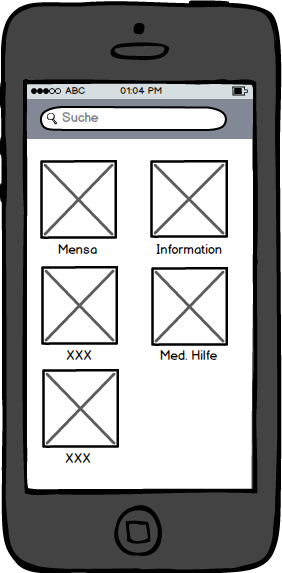
\includegraphics[width=.8\linewidth]{img/menu-mockup.png}
  \label{img:menu-mockup}
  \captionof{figure}{Menü Mockup}
\end{minipage}%
\begin{minipage}[b]{.5\textwidth}
  \centering
  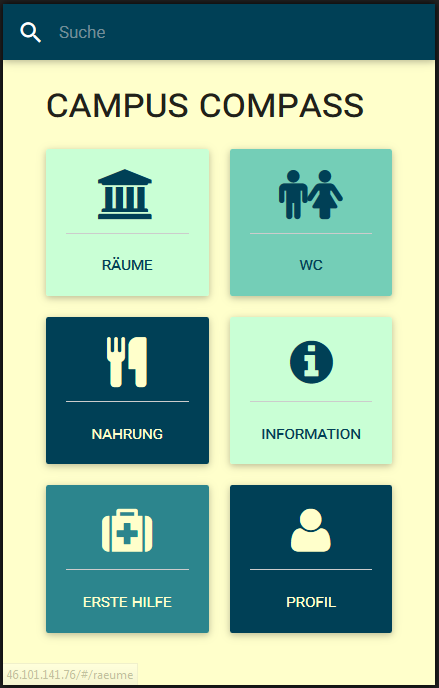
\includegraphics[width=.8\linewidth]{img/menu.png}
  \label{img:menu-first-draft}
  \captionof{figure}{Erster Entwurf Menü}
\end{minipage}
\begin{flushleft}
\begin{minipage}[b]{.5\textwidth}
  \centering
  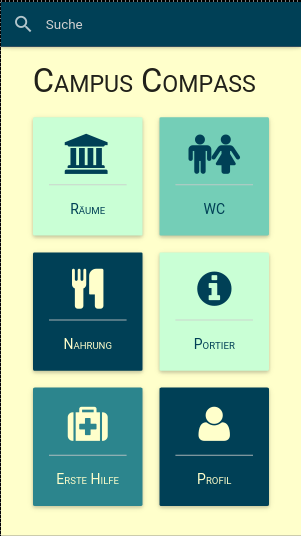
\includegraphics[width=.8\linewidth]{img/menu_final.png}
  \label{img:menu-final}
  \captionof{figure}{Finaler Entwurf Menü}
\end{minipage}
\end{flushleft}
\end{figure}

\begin{figure}[ht]
\centering
\begin{minipage}[b]{.5\textwidth}
  \centering
  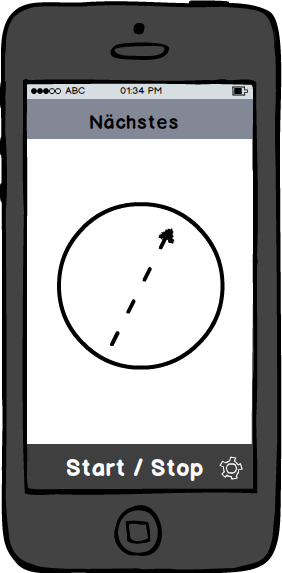
\includegraphics[width=.8\linewidth]{img/navigation-mockup.png}
  \label{img:navigation-mockup}
  \captionof{figure}{\gls{navigation} Mockup}
\end{minipage}%
\begin{minipage}[b]{.5\textwidth}
  \centering
  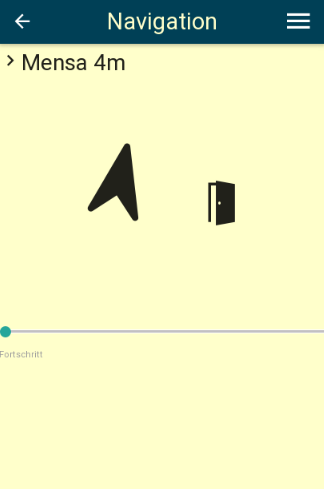
\includegraphics[width=.8\linewidth]{img/navigation.png}
  \label{img:navigation-first-draft}
  \captionof{figure}{Erster Entwurf \gls{navigation}}
\end{minipage}
\begin{flushleft}
\begin{minipage}[b]{.5\textwidth}
  \centering
  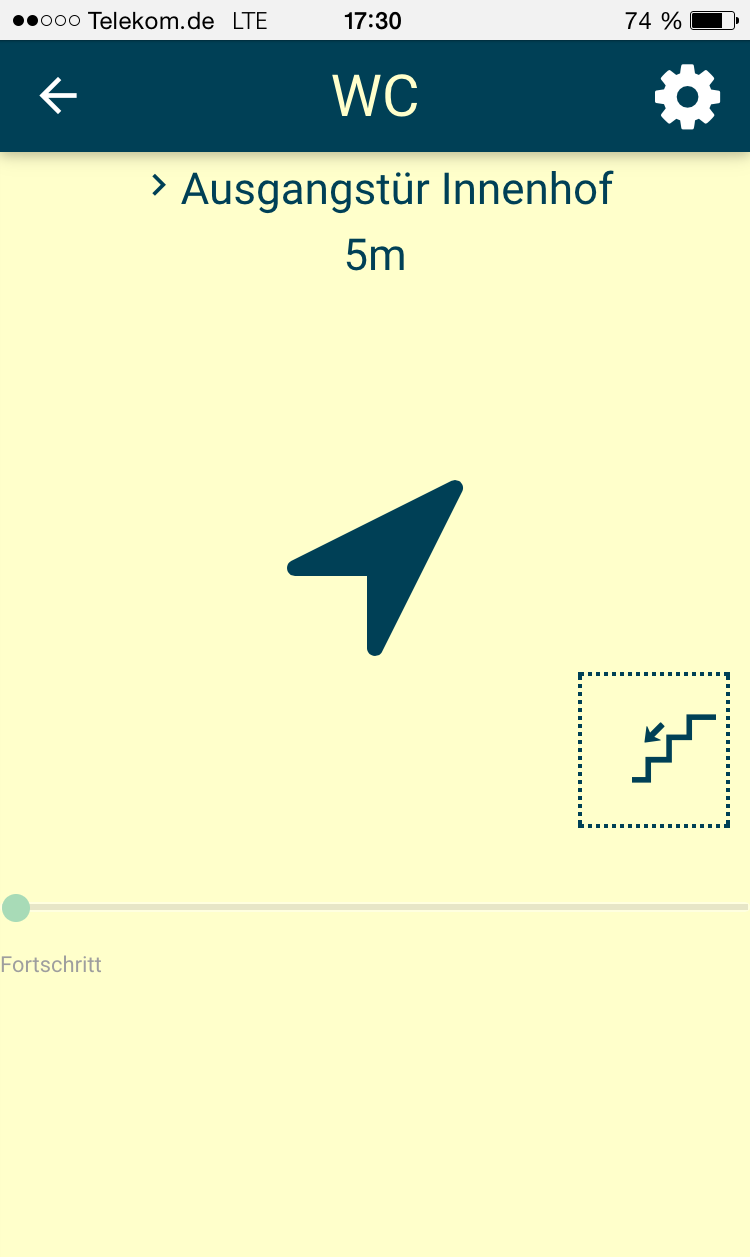
\includegraphics[width=.8\linewidth]{img/navigation2.png}
  \label{img:navigation-second-draft}
  \captionof{figure}{Aktuelle Ansicht \gls{navigation}}
\end{minipage}
\end{flushleft}
\end{figure}

\begin{figure}[ht]
\centering
\begin{minipage}[b]{.5\textwidth}
  \centering
  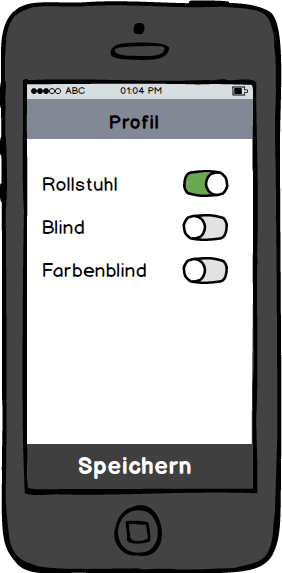
\includegraphics[width=.8\linewidth]{img/profil-mockup.png}
  \label{img:profil-mockup}
  \captionof{figure}{Profil Mockup}
\end{minipage}%
\begin{minipage}[b]{.5\textwidth}
  \centering
  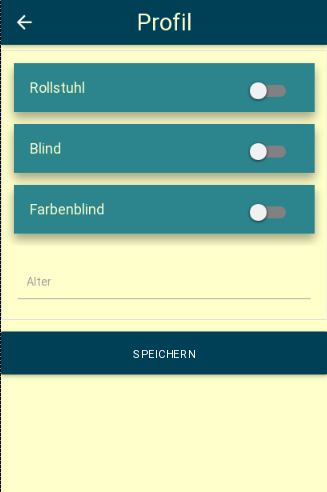
\includegraphics[width=.8\linewidth]{img/profil.png}
  \label{img:profil-first-draft}
  \captionof{figure}{Erster Entwurf Profil}
\end{minipage}
\begin{flushleft}
\begin{minipage}[b]{.5\textwidth}
  \centering
  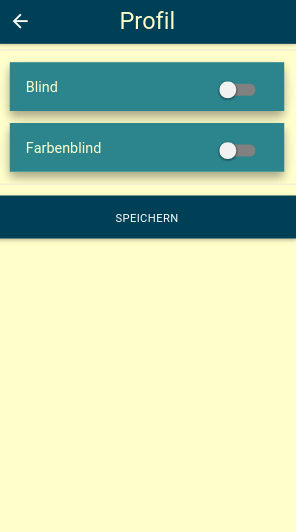
\includegraphics[width=.8\linewidth]{img/profil_final.png}
  \label{img:profil-final}
  \captionof{figure}{Finaler Entwurf Profil}
\end{minipage}
\end{flushleft}
\end{figure}

\begin{figure}[ht]
\centering
\begin{minipage}[b]{.5\textwidth}
  \centering
  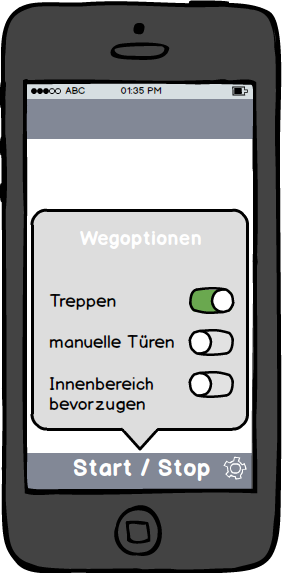
\includegraphics[width=.8\linewidth]{img/wegoptionen-mockup.png}
  \label{img:wegoptionen-mockup}
  \captionof{figure}{Wegoptionen Mockup}
\end{minipage}%
\begin{minipage}[b]{.5\textwidth}
  \centering
  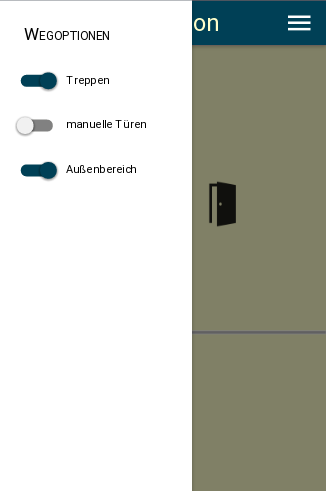
\includegraphics[width=.8\linewidth]{img/wegoptionen.png}
  \label{img:wegoptionen-first-draft}
  \captionof{figure}{Erster \& letzter Entwurf Wegoptionen}
\end{minipage}
\end{figure}